\section{Bridging Small and Large Model Scale Evaluation} \label{sec:rbridge}

\begin{figure}[tb]
    \centering

    \begin{subfigure}[b]{\textwidth}
        \centering
        
\includegraphics[width=0.5\textwidth]{figs/legend_graded.pdf}
        \label{fig:legend}
    \end{subfigure}

    \begin{subfigure}[b]{0.497\textwidth}
        \centering
        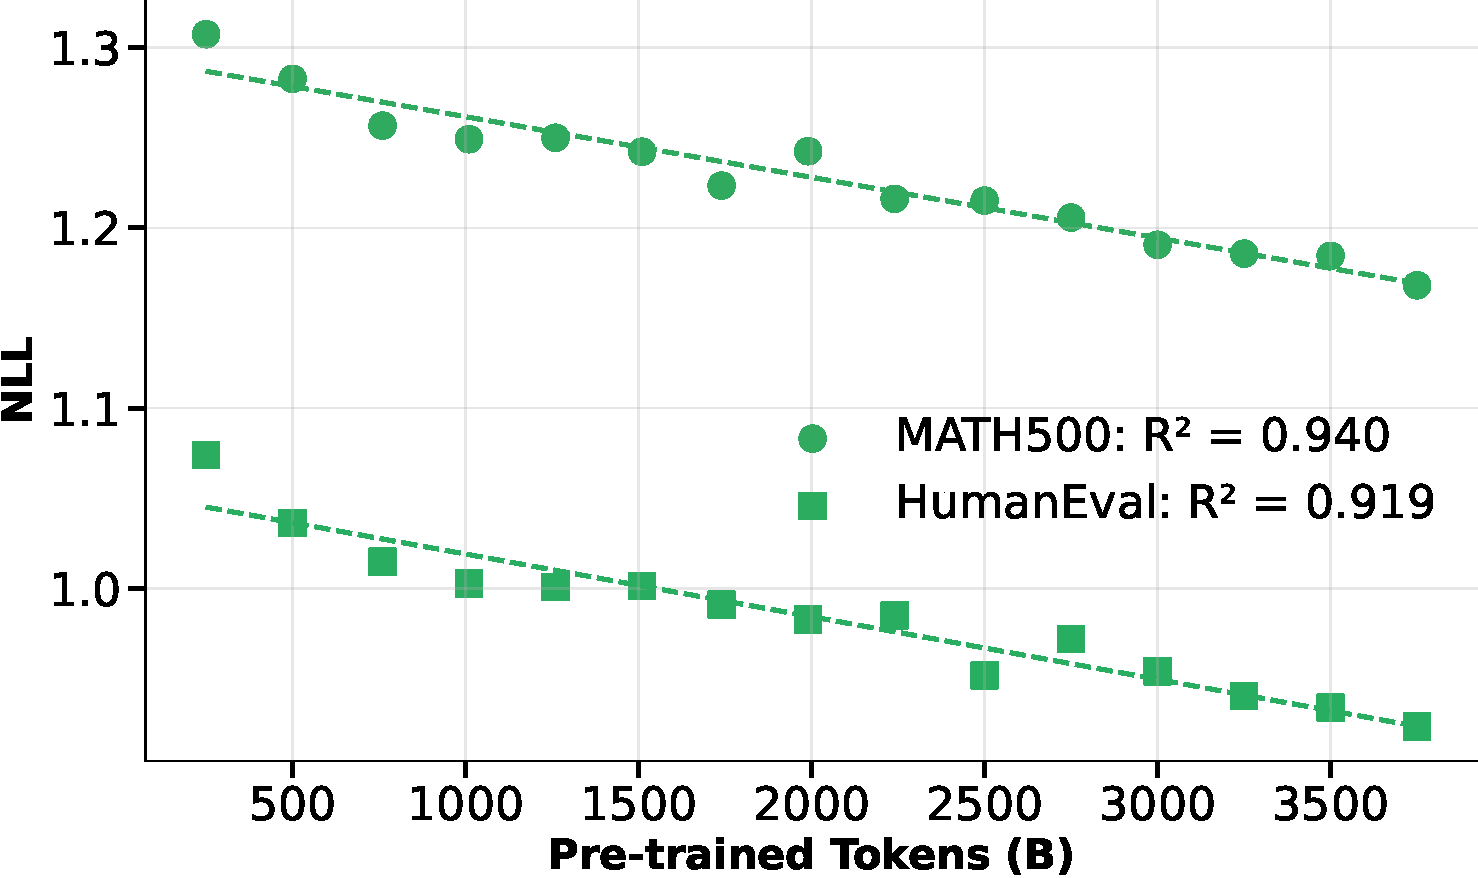
\includegraphics[width=\textwidth]{figs/low_ll_benchmarks.pdf}
        \caption{In-distribution $Y^*$ provides smooth signal.}
        \label{fig:id}
    \end{subfigure}
    \hfill
    \begin{subfigure}[b]{0.497\textwidth}
        \centering
        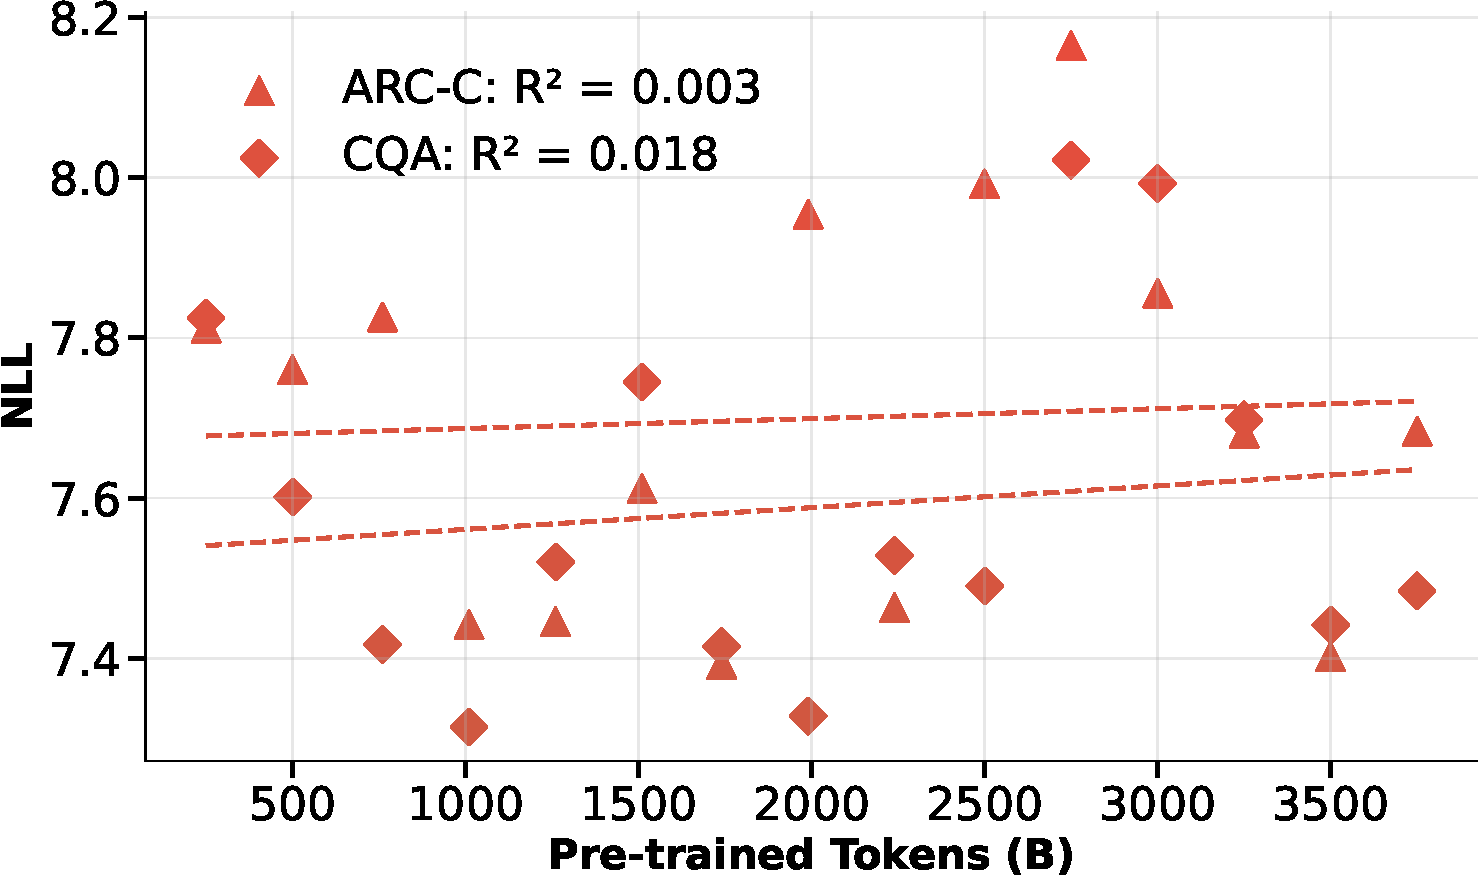
\includegraphics[width=\textwidth]{figs/high_ll_benchmarks.pdf}
        \caption{Out-of-Distribution $Y^*$ provides no signal.}
        \label{fig:ood}
    \end{subfigure}
    \caption{When evaluating a 1B pre-trained model with next token prediction, $\pi^\text{p}(y_\tau \vert x, y^*_{<\tau})$, whether the target $Y^*$ is in-distribution becomes important. All visualized benchmarks demonstrate smooth improvements at larger (13$\times$, 32$\times$) scale with target metric Acc./p@k. For clarity, we visualize the benchmarks in our empirical study with the two smallest and largest average NLL values.}
    \label{fig:idood}
\end{figure}
We find that small models become strong proxies for large models when achieving alignment along two axes: alignment with the pre-training evaluation objective \textbf{(\S\ \ref{sec:limit} (1))}, and alignment with the target task \textbf{(\S\ \ref{sec:limit} (2))}. In response, we introduce our method, \tsc{rBridge} \textbf{(\S\ \ref{sec:align})}.

\subsection{Prior Approach Limitation}\label{sec:limit}

\paragraph{(1) Evaluation Objective Misalignment.} We find that the first limitation of existing approaches is their lack of evaluation objective alignment with $\pi^\text{p}$. This is required as small pre-trained models \textit{lack strong generalization capabilities}. Concretely, \textbf{(a)} Acc. and Pass@K (p@k) is misaligned with the pre-training objective function, and \textbf{(b)} even if we use an objective function aligned evaluation scheme like NLL, we must stay aligned with the pre-trained model's distribution. 

\paragraph{(1.a) Misaligned Evaluation Metric.} Existing target metrics like Acc./p@k are misaligned with the proxy model's next token prediction (NTP) NLL learning objective \citep{brown-etal-1992-class}. \begin{center}
\vspace*{-6mm}

    \begin{minipage}[b]{0.497\textwidth}
        \centering
        \resizebox{\textwidth}{!}{
        \begin{tabular}{lccc}
        \toprule
        \textbf{$Y^*$:} & $\mathcal{D}$ & \textbf{ScB = $R^\phi$ + $A^\phi$}  & \textbf{$R^\phi$} \\
        \midrule
        Min NLL ($\downarrow$)   &\cellcolor{myorange!30} 1.168 & \cellcolor{myred!30} 1.285 & \cellcolor{mygreen!30} 0.925 \\
        Average NLL ($\downarrow$)   &\cellcolor{myorange!30} 1.228 & \cellcolor{myred!30} 1.351 & \cellcolor{mygreen!30} 0.981 \\
        Max NLL ($\downarrow$)   &\cellcolor{myorange!30} 1.307 & \cellcolor{myred!30} 1.405 & \cellcolor{mygreen!30} 1.060 \\
\multicolumn{4}{c}{\cellcolor{gray!10}\textbf{1B $\rightarrow$ 13B}}\\
        Train $R^2$ ($\uparrow$) &\cellcolor{myorange!30}0.861 & \cellcolor{myred!30}0.814 & \cellcolor{mygreen!30}0.886 \\
        Test MAE ($\downarrow$)   & \cellcolor{myorange!30}0.593 & \cellcolor{myred!30}0.637 & \cellcolor{mygreen!30}0.524 \\
\multicolumn{4}{c}{\cellcolor{gray!10}\textbf{1B $\rightarrow$ 32B}}\\
        Train $R^2$ ($\uparrow$) & \cellcolor{myorange!30}0.823 & \cellcolor{myred!30}0.809 & \cellcolor{mygreen!30}0.832 \\
        Test MAE ($\downarrow$)   & \cellcolor{myorange!30}0.815 & \cellcolor{myred!30}0.933 & \cellcolor{mygreen!30}0.739 \\
        \bottomrule
        \end{tabular}
        }
        \captionof{table}{We observe a direct relationship between degree of in-distribution (as presented as NLL) and performance. Best to worst in each row labeled as {\setlength{\fboxsep}{2pt}\colorbox{mygreen!30}{green} \colorbox{myorange!30}{orange}, \colorbox{myred!30}{red}.}} \label{tab:scb}
    \end{minipage}
    \hfill 
    \begin{minipage}[b]{0.497\textwidth}
        \centering
        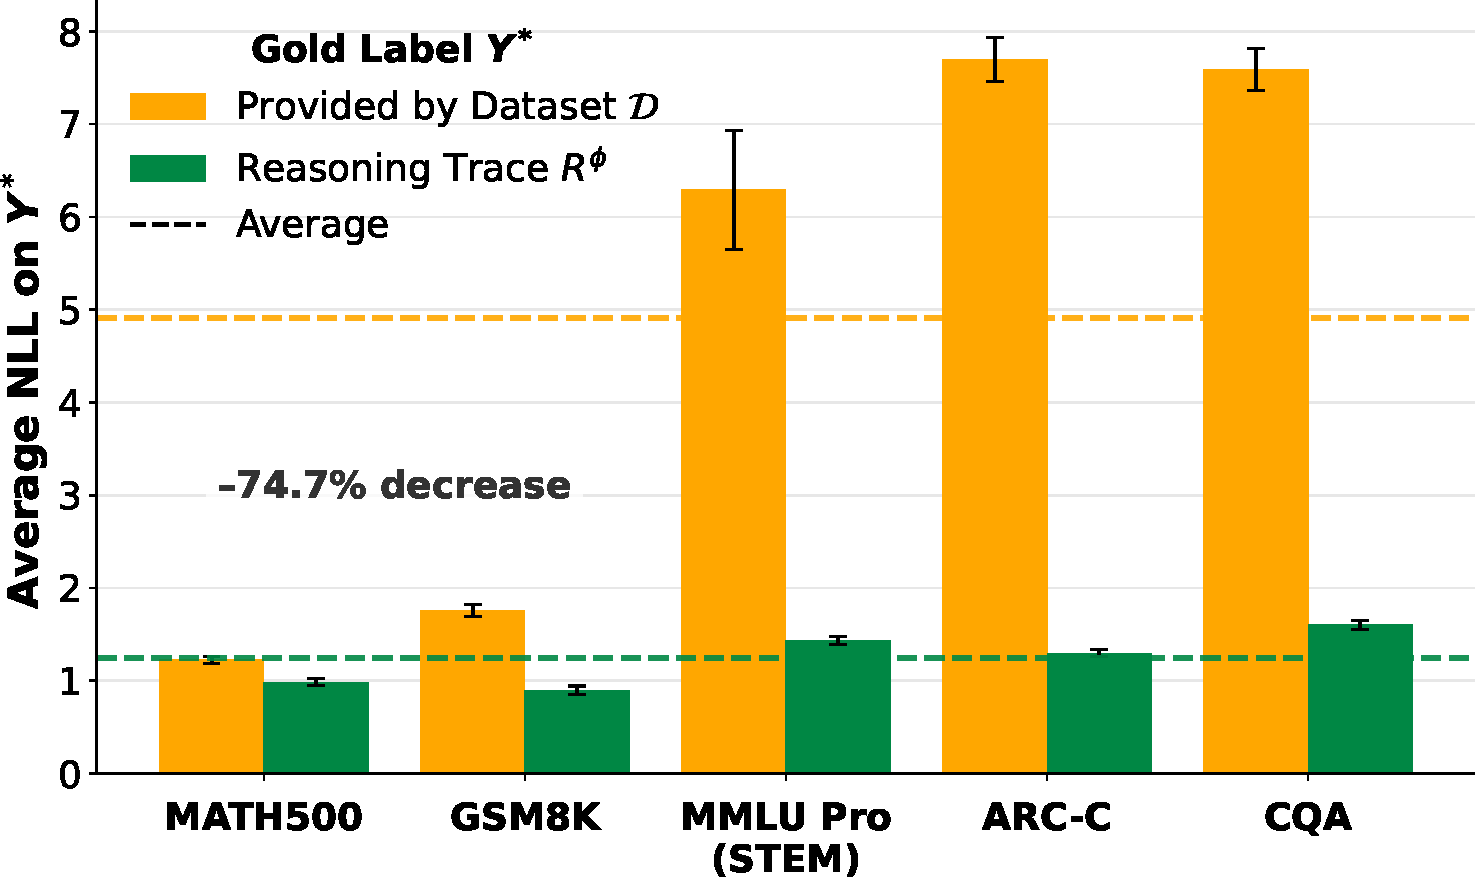
\includegraphics[width=\textwidth]{figs/ll_decrease.pdf}        
        \captionof{figure}{Using reasoning trace $R^\phi$ over benchmark test set's $Y^*$ significantly reduces NLL, suggesting that $R^\phi$ is more in-distribution. Error bars indicate one standard deviation.}\label{fig:scb_clean}
    \end{minipage}
\end{center}
\vspace*{-1mm}Consider Fig. \ref{fig:id}, where NLL shows smooth improvement with correct slope at 1B on MATH500 while Acc. in Fig. \ref{fig:motivation} is noisy and sloping the wrong direction.

\paragraph{(1.b) Not All NLL are Equal: Distributional Alignment.} Furthermore, we find that the quality of the NLL signal hinges on the gold label $Y^*$. We define gold label as the string used for NLL on our proxy model. We observe that it should be closer to the pre-training distribution $p(y_\tau \vert x, y^*_{<\tau}) \sim \pi^\text{p}$ where $x$ is the input, and $\tau$ is the decoded token. Following \cite{arora-etal-2021-types}, \cite{gonen2023demystifying}, we measure how in-distribution (ID) $Y^*$ is via NLL, $-\log(p(Y^*))$. The more out-of-distribution (OOD), the more lacking in signal the proxy model becomes (Fig. \ref{fig:idood}). Benchmarks with an ID $Y^*$ (lower NLL) show smooth and predictable progress at smaller model scale (1B) (Fig. \ref{fig:id}). Contrarily, benchmarks with OOD $Y^*$ (higher NLL) is at least as noisy as the target metric Acc. (Fig. \ref{fig:ood}). 

We also observe this distributional misalignment in ScalingBench (ScB; \cite{xiao2024densing,team2025minicpm4}). ScB proposes we set the reasoning trace $R^\phi$ \citep{NEURIPS2022_9d560961} and the final answer label $A^\phi$ of a frontier model $\pi^\phi$ as $Y^*$. ScB's gold labels include formatting artifacts like ``$\backslash$n", ``Final Answer:", and ``I hope it is correct." that rarely appear in pre-training data, making them OOD, hurting proxy performance (Tab. \ref{tab:scb}). The proxy evaluation protocol is detailed in \textbf{\S\ \ref{sec:protocol} (ii)}. 

% For instance, in ScB's MATH $Y^*$ their final answer label is includes ``$\backslash$n", ``Final Answer:", and ``I hope it is correct." which does not commonly occur in the pre-training corpora. Therefore, in the case of ScB provided MATH $Y^*$, the NLL is more OOD (Tab. \ref{tab:scb}). Our preliminary study shows that this hurts proxy performance (Tab. \ref{tab:scb}).

\paragraph{(2) Target Task Alignment of Gold Label $Y^*$ and at the Token Level.} Secondly, we hypothesize that the evaluation scheme should be task aligned. Here, target task refers to, e.g., correctly solving math problems for GSM8K \citep{cobbe2021training}, and MATH500 \citep{hendrycks2021math}. Ensuring that $Y^*$ is aligned with the target task is necessary to fulfilling our \textit{ultimate} goal of proxying task performance at large scale. While we could achieve maximal ID by setting the greedy decoded tokens of $\pi^\text{p}(y_\tau \vert x, y^*_{<\tau})$ as $Y^*$, this would provide no signal, as it would fail to be task aligned. 

We further observe that standard NLL on $Y^*$ does not distinguish between tokens that are important for task alignment, and others that are less task critical. Consider, Fig. \ref{fig:rbridge}, where frontier model $\pi^\phi$ decoding produces both {\color{mygreen}\textbf{task critical}} and {\color{myorange}\textbf{formatting/creative}} tokens. For example, newlines and numbering are not essential, while steps like ``sum modulo 9’’ are crucial. To further achieve task alignment, tokens should not be arbitrarily given equal weight as is in NLL. 

\subsection{rBridge: Improving Evaluation Objective Alignment and Task Alignment} \label{sec:align}
  
\paragraph{Reasoning Trace $R^\phi$ as $Y^*$.} We show that using only the reasoning trace $R^\phi$ of a frontier model $\pi^\phi$ as $Y^*$ satisfies both being \textbf{(1)} ID and \textbf{(2)} task alignment. \textbf{(1)} We hypothesize that $R^\phi$ is more distributionally aligned (ID) with the pre-training distribution comprised predominantly of a collection of continuous long texts \citep{NEURIPS2024_370df50c,kydlicek2025finepdfs}. We verify this empirically in Fig. \ref{fig:scb_clean}, where we visualize average NLL across 250 to 3750B trained tokens on a 1B model, on the provided $Y^*$ by the benchmark dataset $\mathcal{D}$ against the frontier model $\pi^\phi$ generated $R^\phi$. We observe an average NLL decline of 74.7\% when using $R^\phi$ across five reasoning benchmarks, providing supportive evidence that $R^\phi$ is more ID. \textbf{(2)} $R^\phi$ is well aligned with the target task as $R^\phi$ is the reasoning trace that leads to the correct final answer for Acc./p@k. Intuitively, evaluating how well the model $\pi^\text{p}$ reasons towards the final answer is a good ID proxy for achieving the target Acc./p@k. Empirically, using only $R^\phi$ achieves the best relationship on MATH500 which we are able to replicate as the exact ScB $Y^*$ gold labels have been released for MATH500 (Tab. \ref{tab:scb}).  

 % We wish to refine $Y^* := R^\phi$ automatically so that tokens that are more task aligned are given more weight.

\paragraph{Weighted NLL on $R^\phi$'s Tokens for 
Further Task Alignment.} \tsc{rBridge} takes a final step for further task alignment by weighting each token by its level of task-alignment. We hypothesize that frontier model token probability $p^\phi(\text{token}_i) \sim \pi^\phi$ provide automatic task-alignment weights:

\begin{equation}\label{eq:rbridge_nll}
    \text{\tsc{rBridge} NLL}(\text{token}_i):=  \underbrace{-\text{log}(p^\text{p}(\text{token}_i))}_{\text{standard NLL}} \cdot 
    \underbrace{\frac{1}{\vert \text{token}_i \vert} \sum_{\text{letter} \in \text{token}_i} p^\phi(\text{letter})}_{\text{Automatic tokenizer-agnostic task-alignment weight}
    }.
\end{equation}

Our method weighs each token $i$'s NLL by the frontier model's confidence in that token $p^\phi(\text{token}_i)$. To handle different tokenizers, we average letter-level probabilities within each token. Finally, we apply MinMax normalization \citep{witten2002data} on the weight factor in Eq. (\ref{eq:rbridge_nll}) to amplify the effect. Consider Fig. \ref{fig:rbridge} for an intuitive visualization of Eq. (\ref{eq:rbridge_nll}) with the MinMax normalized form unpacked in full. The pseudocode and prompt is available at Appendix \ref{app:pseudocode}.

% Finally, to amplify the effect of the task-alignment weight, we MinMax normalize \citep{witten2002data} it. We found this useful as $p^\phi(\text{token})$, and in turn $p^\phi(\text{letter})$ values taken via greedy decoding \citep{NIPS2014_5a18e133} naturally lead to probability distribution skewed towards high values. The pseudocode and prompt is available at Appendix \ref{app:pseudocode}.

% Note that we use their few-shot prompting format to evaluate NLL.

% In short, we evaluate performance using $K$-Fold Train $R^2$ and Test MAE.

% Such extreme non-task aligned $Y^*$ would provide the equivalent NLL across all scenarios. 

%as using free-form generation-based metrics like Acc. and pass@k leads to worse performance as error accumulates \citep{NIPS2015_e995f98d,ranzato2015sequence}. Intuitively, NTP is a more forgiving metric for the weak proxy model $\pi^\text{p}$ as at each decoding step $t$, the provided context $<t$ is the gold answer. We denote gold label for NTP as $Y^*$.

% We first overcome the inherent weakness of proxy models, being small and pre-train-only, by aligning the evaluation scheme with the pre-training objective. While larger models embody emergent behavior, i.e., achieving stable reasoning performance scores, we find that the best way to achieve reliable signals at small scale is by using the same metric the proxy pre-trained model $\pi^\text{p}$ was trained on. Therefore, we employ next token prediction (NTP) evaluation via average negative log likelihood per token (henceforth referred to as NLL; \cite{brown-etal-1992-class}). 

% We retrieve $R^\phi$ by prompting $\pi^\phi$ to generate a reasoning trace $R^\phi$ and final answer $A^\phi$. We discard $A^\phi$ and set $Y^* := R^\phi$.

% We qualitatively observe why benchmarks like ARC-C and CQA's $Y^*$ are significantly more OOD. As these benchmarks are multiple-choice question-based, the target $Y^*$ becomes the multiple-choice symbol, e.g., ``B" \citep{eval-harness}, or a short string, e.g. ``The Sun makes heat." \citep{gu-etal-2025-olmes}. In turn, $Y^*$ is distant from the pre-trained distribution of $\pi^\text{p}(y_\tau \vert x, y^*_{<\tau})$. Intuitively, as the pre-training corpora is predominantly a collection of continuous long texts \citep{NEURIPS2024_370df50c,kydlicek2025finepdfs}, such question-and-short-answer formats are rare in the corpora. 

% allowing the weight factor range to transform from $[a, b]$ to $[0, 1]$ where $a\geq0$ and $b\leq1$. min($\cdot$) and max($\cdot$) search space is set to the entire test set's evaluated tokens. 

% Straightforward assignment $p^\phi(\text{letter}) := p^\phi(\text{token})$, where letter $\in$ token, provides letter-level weights from the frontier-level model $\pi^\phi$. Letter-level is the most reasonable choice as this is the atomic unit of a token; meaning, we can re-map $p^\phi(\text{letter})$ back to any different tokenizer's token. As seen in Eq. \ref{eq:rbridge_nll}, this is achieved by finding the mean $p^\phi(\text{letter})$  across all letters composing the token. This weight factor is bounded by $[0, 1]$. A concretely example is visualized in Fig. \ref{fig:rbridge}.